\section{Lecture 10: Cache Coherence}
When using cache in multiprocessor systems, different processor may access the same data in memory. This gives us a problem with that we have multiple copies of the same data in different caches. This is known as the \textbf{cache coherence} problem.

\subsection{Introduction}
How can we assure that the other processors get the update in another processors cache, and that we don't overwrite some memory that is critical?
We must ensure that \textbf{WRITE} operations is carefully coordinated.
\subsubsection{Write Through}
\textbf{Write through}: All write operations are made to main memory as well as to the cache, ensuring that main memory is always valid.

But there are some problems with this:
\begin{itemize}
\item Can slow down the main memory access since we need to write a lot, and this takes time, but since the write percentage is only about 15\% its okay.
\item Inconsistency can occur unless other caches monitor the memory traffic or receive some direct notification of the update.
\item Multiple CPUs must therefore monitor main memory traffic to keep local cache up to date.
  \begin{itemize}
  \item This may lead to a lots of traffic and monitoring activities.
  \end{itemize}
\end{itemize}

\subsubsection{Write Back}
\textbf{Write back}: Write operations are usually made only to the cache. Main memory is only updated when the corresponding cache line is flushed from the cache.
\begin{itemize}
\item We update a bit when the cache is updated.
\item If we need to replace a bit, we look at the bit to see if the cache has been updated and it needs to be saved to the main memory.
\end{itemize}

It is clear that a write-back policy can result in inconsistency. If two caches contain the same line, and the line is updated in one cache, the other cache will unknowingly have an invalid value. Subsequent reads to that invalid line produce invalid results. Therefore we need additional techniques.
\subsubsection{Software Solutions}
Here we deal with the problem during \textbf{compile time}, this gives us time to determine which data item that may become unsafe for caching, (e.g. global parameters are typical).

We can either mark these data entries so that they are not cached. This is too conservative, because a shared data structure may be exclusively used during some periods and may be effectively read-only during other periods. It is only during periods when at least one process may update the variable and at least one other process may access the variable that cache coherence is an issue.

Alternatively we can determine the unsafe periods and insert code to enforce cache coherence.

Pros with software solutions:
\begin{itemize}
\item Avoid the need for additional hardware circuitry and logic by relying on the compiler and operating system to deal with the problem.
\end{itemize}

Cons with software solutions:
\begin{itemize}
\item We may get inefficient cache utilization and we might therefore get low performance of the memory system.
\end{itemize}

\subsubsection{Hardware Solutions}
Hardware-based solutions are generally referred to as cache coherence protocols. These solutions provide dynamic recognition at run time of potential inconsistency conditions. Because the problem is only dealt with when it actually arises, there is more effective use of caches, leading to improved performance over a software approach. In addition, these approaches are transparent to the programmer and the compiler, reducing the software development burden.

In general, hardware schemes can be divided into two categories: \textbf{directory protocols} and \textbf{snoopy protocols}.

\subsection{Directory protocols}
Here we have a collections that maintain information about where copies of lines reside. Typically a centralized controller that is part of the main memory controller and a directory stored in the main memory. This works as following:

\begin{itemize}
\item When an individual cache controller makes a request, the centralized controller checks and issues necessary commands
\item Instead of reading data from the main memory we instead may fetch data from another cache where the data have been updated.
\item It keeps the state information up to date. Therefore, every local action that can affect the global state of a line must be reported to the central controller.
\item Grants exclusive memory access to processor, by forcing all other processor to invalidate its copy.
\item If a processor tries to read a line that is exclusively granted to another processor, it will send a miss notification to the controller. The controller then issues a command to the processor holding that line that requires the processor to do a write back to main memory. The line may now be shared for reading by the original processor and the requesting processor.
\end{itemize}

Directory schemes suffer from the drawbacks of a central bottleneck and the overhead of communication between the various cache controllers and the central controller. However, they are effective in large-scale systems that involve multiple buses or some other complex interconnection scheme.
\subsubsection{Cache Coherence Operations}
\todo{byt ut denna sektion mot ett exempel kanske.}
\subsection{Snoopy protocols}
Snoopy protocols distribute the responsibility for maintaining cache coherence among all of the cache controllers in a multiprocessor. A cache must recognize when a line that it holds is shared with other caches. When an update action is performed on a shared cache line, it must be announced to all other caches by a broadcast mechanism. Each cache controller is able to “snoop” on the network to observe these broadcasted notifications, and react accordingly.

Snoopy protocols are ideally suited to a bus-based multiprocessor, because the shared bus provides a simple means for broadcasting and snooping. But this also means that we get increased bus traffic.

Two basic approaches to the snoopy protocol have been explored, \textbf{write invalidate} and \textbf{write update} (or write broadcast). Neither of these two approaches is superior to the other under all circum- stances. Performance depends on the number of local caches and the pattern of memory reads and writes. Some systems implement adaptive protocols that employ both write-invalidate and write-update mechanisms.
\subsubsection{Write Invalidate SP}
With a write-invalidate protocol, there can be multiple readers but only one writer at a time. Initially, a line may be shared among several caches for reading purposes. When one of the caches wants to perform a write to the line, it first issues a notice that invalidates that line in the other caches, making the line exclusive to the writing cache. Once the line is exclusive, the owning processor can make cheap local writes until some other processor requires the same line.

The write-invalidate approach is the most widely used in commercial multiprocessor systems, such as the Pentium 4 and PowerPC. It marks the state of every cache line (using two extra bits in the cache tag) as modified, exclusive, shared, or invalid. For this reason, the write-invalidate protocol is called MESI.


\subsubsection{Write Update SP}
With a write-update protocol, there can be multiple writers as well as multiple readers. When a processor wishes to update a shared line, the word to be updated is distributed to all others, and caches containing that line can update it.

But it may generate many unnecessary updates if a processor:
\begin{itemize}
\item Reads a value without ever needing it. 
\item Updates a value several times before it is read by other processors. 
\end{itemize}

\subsubsection{MESI State Transition Diagram}
\begin{figure}[H]
  \centering
  \scalebox{0.45}{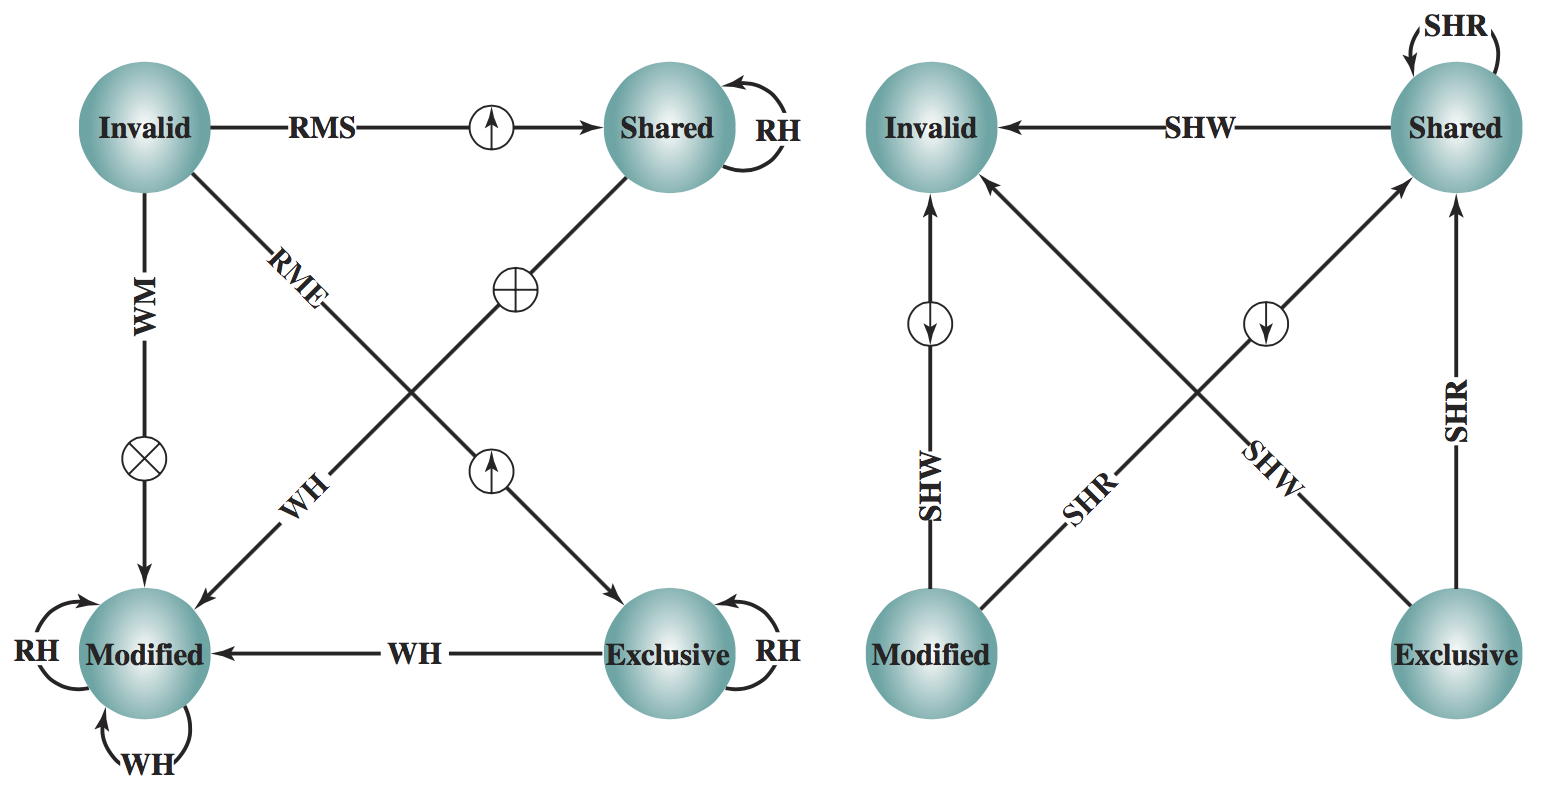
\includegraphics{img/mesi-states.png}}
  \scalebox{0.45}{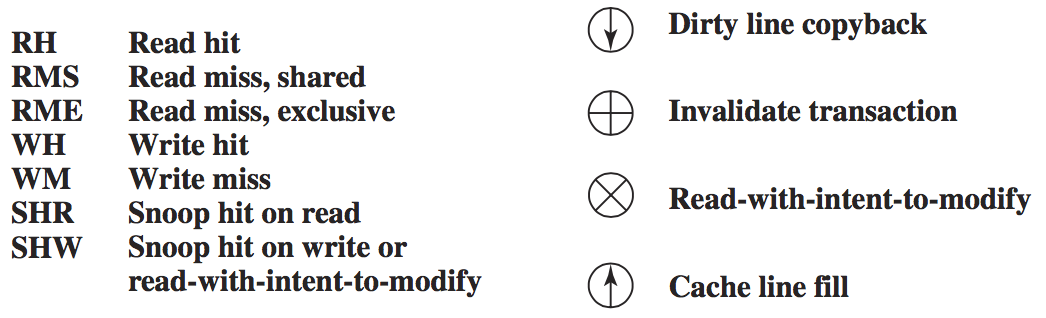
\includegraphics{img/mesi-descriptions.png}}
  \caption{MESI State Diagram.}
  \label{fig:mesi}
\end{figure}
\todo{UNDERSTAND THIS}
\subsubsection{Invalidate vs. Update Protocols}
\begin{itemize}
\item An update protocol may generate many unnecessary cache updates, so if two processors make interleaved reads and updates to a variable, an update protocol is better.
\item Both protocols suffer from false sharing overheads, which means that when two words are not shared but they lie within the same cache line.
\item Most modern machines use invalidate protocols, since we have usually the case of one writer and many readers.
\end{itemize}

\subsubsection{Directory vs. Snoopy Schemes}
\begin{itemize}
\item Snoopy caches
  \begin{itemize}
  \item Each coherence operation is sent to all processors.
  \item It generates large traffic, which is an inherent limitation.
  \item Easy to implement on a bus-based system.
  \item Not feasible for machines with memory distributed across a large number of sub-systems.
  \end{itemize}
\item Directory caches
  \begin{itemize}
  \item The need for a broadcast media is replaced by the directory.
  \item The additional information stored in the directory may add significant overhead.
  \item The underlying network must be able to carry all the coherence requests.
  \item The directory is a point of contention, therefore, distributed directory schemes are often used.
  \end{itemize}
\end{itemize}
\subsection{L1-L2 consistence}
When we have several layers of cache we can't use snoopy protocols since the L1 cache won't be connected to a bus (L2 is connected). The solution is to extend cache coherence protocols to L1 cache, which means that the L1 line must keep track of the corresponding state of the L2 cache, and L1 should write-through to L2. If L1 uses write-back, we ge a more complex solution.

But this requires the following:
\begin{itemize}
\item L1 must be a subset of L2
\item The associativity of L2 must be equal or greater than that of L1.
\end{itemize}

\subsubsection{Alpha-Server 4100}
\begin{itemize}
\item Four-processor shared-memory symmetric multiprocessor
  system.
\item Each processor has a three-level cache hierarchy:
  \begin{itemize}
  \item L1 consists of two direct-mapped on-chip caches, onefor instruction and one for data.
    \begin{itemize}
    \item Write-through to L2 with a write buffer.
    \end{itemize}
  \item L2 is an on-chip three-way set associative cache with write-back to L3.
  \item L3 is a off-chip direct-mapped cache with write-back to main memory.
  \end{itemize}
\end{itemize}
